\vspace*{1.5pc}

In Sec.~\ref{sec:pureWDM}, I detailed the results yielded by our likelihood analysis of the Ly-$\alpha$ forest power spectrum in two projects I investigated in a pure dark matter cosmology: right-handed neutrinos as either warm (in absence of net lepton asymmetry) or cool (in presence of $\mathcal{L}>0$) dark matter. In both cases, I assume that all of dark matter is made of a single type of particle. When constraining the mass of left-handed neutrinos through $\sum m_\nu$, we assume that neutrinos are a hot component mixed with a generic cold dark matter particle. In Sec.~\ref{sec:lcdmnu}, I detail the results on this C+HDM cosmology. I also present the results on the mass and relative abundance of warm dark matter particles assuming, likewise, a C+WDM context in Sec.~\ref{sec:cwdm_flux} below. \\

\subsection{Cold+Warm Dark Matter}
\label{sec:cwdm_flux}

In this subsection, I go over the results of our analysis on cold plus warm dark matter cosmologies. As was introduced in Sec.~\ref{sec:CAMB} and specifically Sec.~\ref{sec:cwdm_linear}, the two parameters relevant to this set of cosmologies are the rest mass of the warm component (the cold component being assumed infinitely --- or rather, undeterminedly --- heavy) and its relative abundance with respect to the total dark matter density. I work under the asumption that $\Omega_{\mathrm{dm}} h^2 = 0.26142 \times 0.675^2$ is dichotomised into $0 \leqslant F_{\mathrm{wdm}} \leqslant 1$ of a warm component\footnote{which may be anything from a generic particle, to thermal relics or sterile neutrinos, so long as the rest mass is in the keV ball-park} and $1 - F_{\mathrm{wdm}}$ of the cold component. The fractional abundance therefore acts like an interpolating dial between the two limiting cases: pure cold ($F_{\mathrm{wdm}} = 0$) and pure warm ($F_{\mathrm{wdm}} = 1$) dark matter. This was illustrated in Fig.~\ref{fig:pk_cwdm}, with $F_{\mathrm{wdm}}$ controlling the height of the small-scale plateau of the linear transfer function. Since there is a bijection between NRP sterile neutrino and thermal relic mass, I'll quote masses in terms of $m_x$ for the sake of simplicity.\\

\begin{figure}
\begin{center}
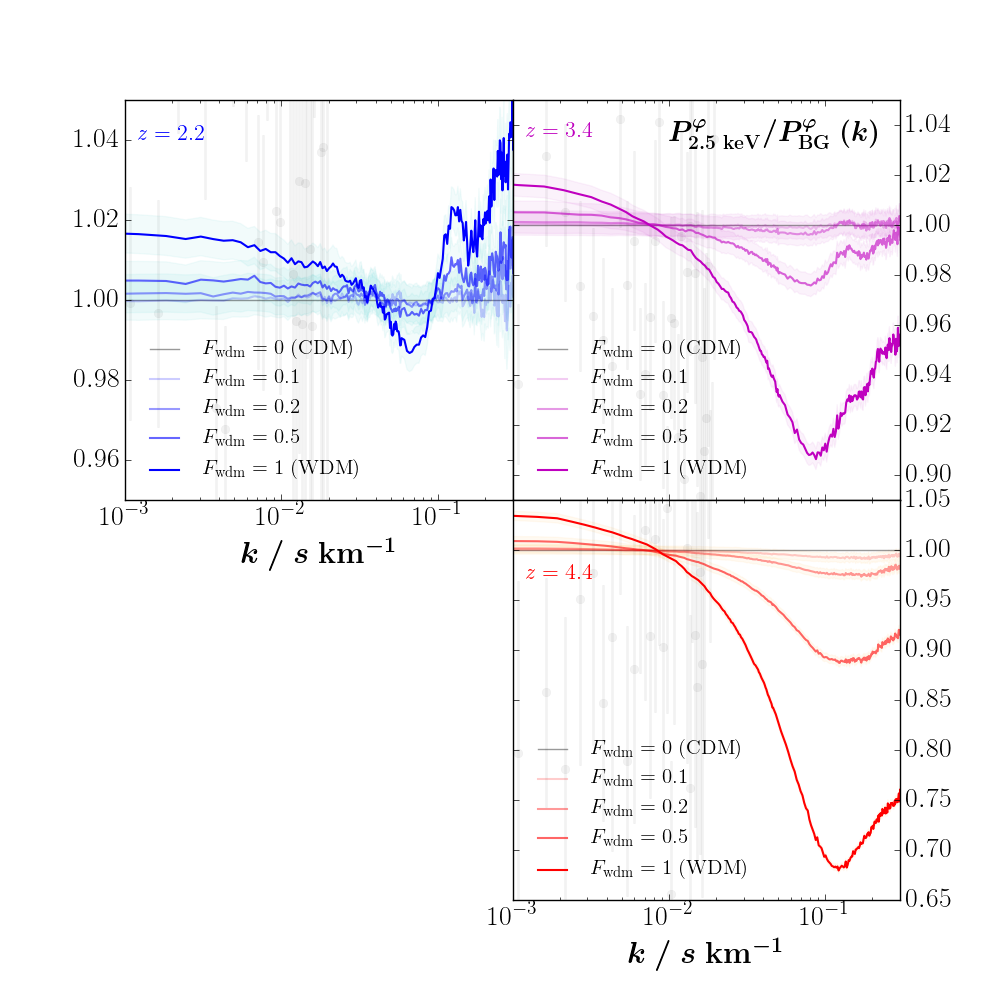
\includegraphics[width=0.85\columnwidth]{CWDM_PkLya_25keV_lya.png}
\caption{Flux power spectra of $m_x = 2.5~\mathrm{keV}$ thermal relics as the warm component of a C+WDM cosmology, normalised by that of the benchmark CDM model ($F_{\mathrm{wdm}} = 0$) for $F_{\mathrm{wdm}} = 0\%~ (\mathrm{pure ~cdm}), 10\%, 20\%, 50\%$ and $100\%$ (pure WDM). Top left, top right and bottom right display the power spectra at redshift $z=2.2, 3.4$ and $4.4$ respectively. SDSS/BOSS DR9 Ly-$\alpha$ power spectrum data is superimposed as light grey errorbars.}
\label{fig:cwdm_25keV}
\end{center}
\end{figure}

In Fig.~\ref{fig:cwdm_25keV}, I highlight the effect of the relative abundance parameter on the flux power spectrum --- this time a unidimensional, non-linear probe --- at a fixed mass. The overall behavior is consistent with the linear case: the less abundant the warm component is with respect to the total dark matter density, the more consistent the power spectrum is with the benchmark CDM case, \textit{i.e.} the \emph{best guess} configuration. It appears there is a clear monotoneous evolution from the pure cold to the pure warm dark matter limit cases as one increases the value of $F_{\mathrm{wdm}}$, at least on the relevant scales $k \lesssim 0.08~s~\mathrm{km}^{-1}$. In this regard, the high-resolution Ly-$\alpha$ data is suited to distinguish between C+WDM models, with the proviso that several values of $\left( m_x, F_{\mathrm{wdm}} \right)$ may yield a similar flux power spectrum. It is therefore expected that the 2D likelihood function in the $\left( \mathrm{keV}/m_x, F_{\mathrm{wdm}} \right)$ plane exhibits a symmetric axis. Indeed, the authors of \cite{BLR09} showed that the probability distribution in this plane is highly non-Gaussian, with both $F_{\mathrm{wdm}} = 0$ and $\mathrm{keV}/m_x = 0$ axis being the best guess CDM model. It's less evident that the SDSS/BOSS data alone can manage to distinguish between C+WDM models, as the size of the grey errorbars in Fig.~\ref{fig:cwdm_25keV} with respect to the difference between the different curves suggest, apart form the $\sigma_8$ re-normalisation plateau at large scale. It is also apparent that the higher redshift bins have the higher constraining power since the departure from CDM is more pronounced. However, higher redshift data has higher statistical uncertainty due to low object count. It is unclear whether the very small scale ($k \gtrsim 0.1~s/\mathrm{km}$) behavior are due to non-linear effects or simulation artefacts. No dedicated convergence tests where performed down to this precision to investigate this effect. In any case, this particularity affects scales much smaller than what can be resolved with the Ly-$\alpha$ flux power spectrum at hand. \\

\subsubsection{Constraints on $m_x$ and $F_{\mathrm{wdm}}$}

The probability distribution in the $(F_{\rm{wdm}},m_x)$ plane  being strongly non-Gaussian, a Taylor expansion in either of these two parameters would not provide  accurate results. We therefore extend the method described in~\cite{Borde2014, Palanque2015a, Palanque2015b, Baur16} in the following way. We use the likelihood of those works, based on the second-order Taylor expansion, to capture the dependence  of the Ly-$\alpha$ flux power spectrum with the cosmological and astrophysical variables of Table~\ref{tab:parameter_values}, and to model identified nuisance parameters accounting for IGM thermal state modeling, re-ionization redshift, spectrometer noise, and simulation uncertainties. 
To capture the dependence with $F_{\rm{wdm}}$ and $m_x$, I produced a suite of 28 C+WDM simulations with non-zero $(F_{\rm{wdm}},m_x)$ enumerated in Tab.~\ref{tab:cwdm_grid} while all other parameters are set to their \textit{best-guess} value in Table~\ref{tab:parameter_values}. 
For each of the C+WDM simulations, a $\chi^2$ is computed with respect to the $35 \times 12$ $P_\varphi(k, z)$ data points from the BOSS DR9, assuming a Gaussian distribution for the Hubble parameter, $h=0.673 \pm 0.010$ (Planck 2015), and minimizing over all the parameters of the likelihood described in Sec.~\ref{sec:methodology}. I use a cubic spline interpolation routine within the positions of the 28 C+WDM models in the $\left( \mathrm{keV}/m_x, F_{\mathrm{wdm}} \right)$ plane to predict the probability distribution at any point in the whole parameter spacee, which I feature in Fig.~\ref{fig:chi2_WF}. \\

\begin{figure}
\begin{center}
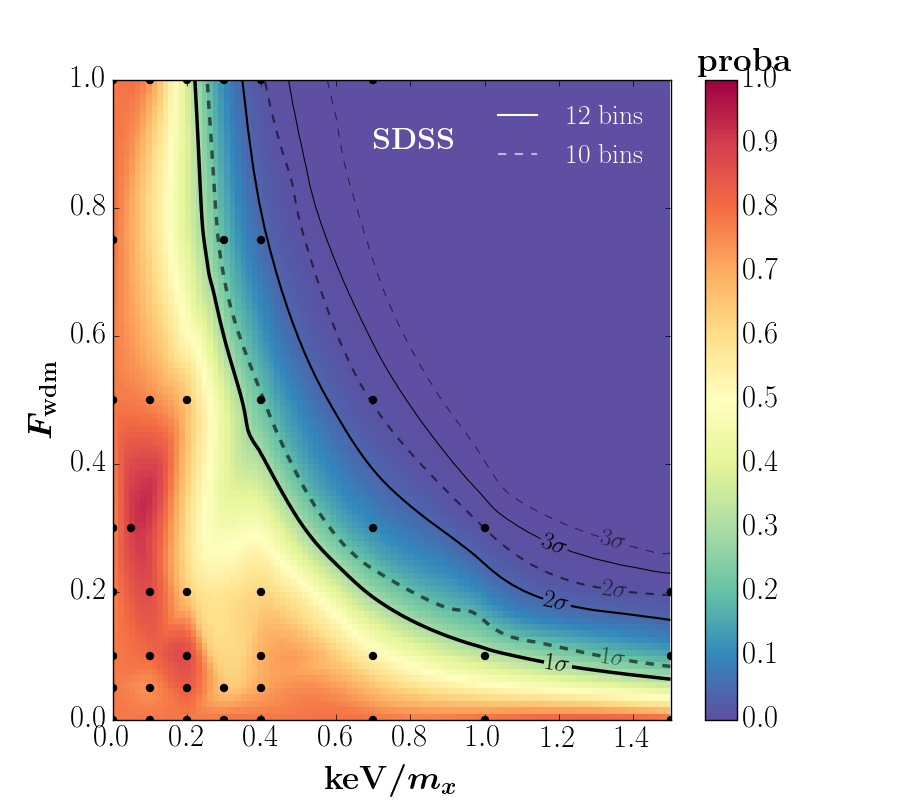
\includegraphics[width=0.55\columnwidth]{RPSN/Chi2_WF_boss.png}~%
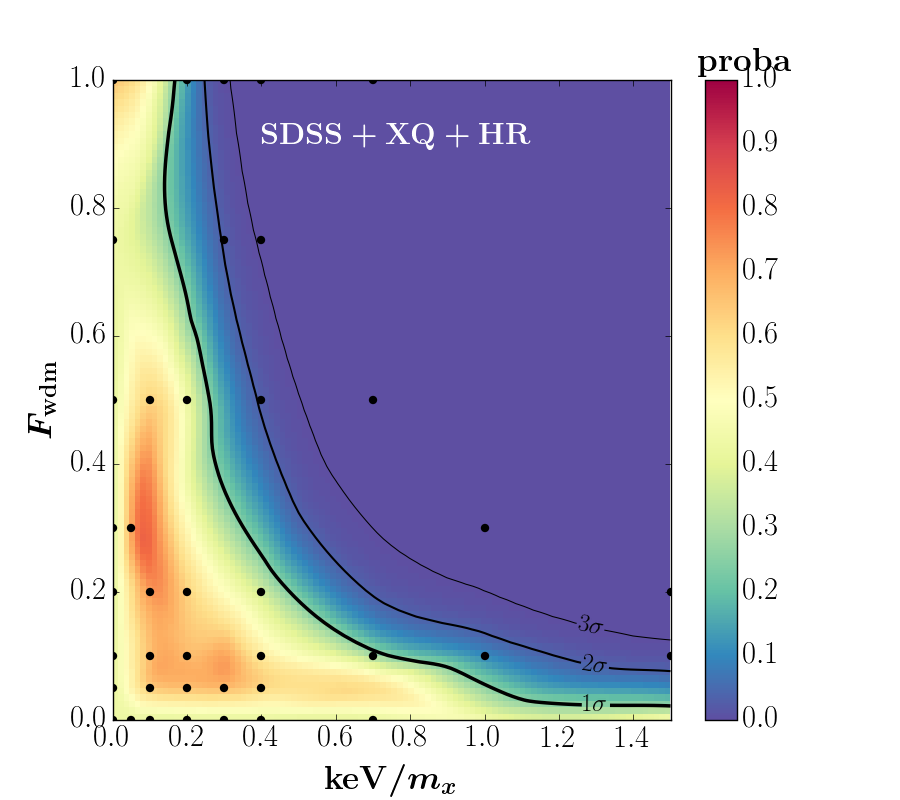
\includegraphics[width=0.55\columnwidth]{RPSN/Chi2_WF_bossxqhr.png}
\caption{Our set of C+WDM hydrodynamical simulations mapped as black dots on
    our grid of ($\mathrm{keV}/m_x$, $F_{\rm{wdm}}$). Note the points
    corresponding to either $F_{\rm{wdm}}=0$ or $\mathrm{keV}/m_x=0$ all
    correspond to the \textit{best guess} model that assumes a CDM
    cosmology. The color scheme reflects the probability function defined in
    Eq.~\ref{eq:proba}. \textbf{Left:} bounds based on the SDSS/BOSS data
    only. Solid curves are 1, 2 and 3$\sigma$ CL contours using all 12
    redshift bins, while the dashed curves materialize the contours when
    excluding the 2 highest redshift bins ($z=4.2$ and $4.4$) in the likelihood. \textbf{Right:}
    combined SDSS/BOSS (all 12 redshift bins) + XQ + HR data set.}
\label{fig:chi2_WF}
\end{center}
\end{figure}


The $\chi^2$ values we obtain along the $F_{\mathrm{wdm}}=1$ axis are in excellent agreement with those of the pure WDM models I ran in Sec.~\ref{sec:pureWDM} and published in \cite{Baur16} and \cite{Yeche17}. The bounds shown in Fig.~\ref{fig:chi2_WF} at $2\sigma$ are expectedly weaker than the ones reported previously since they are computed in the full two-dimensional analysis in the ($\mathrm{keV}/m_x$, $F_{\rm{wdm}}$) plane. Thermally decoupled relics as light as $m_x \geqslant 0.7~\mathrm{keV}$ are consistent with Ly-$\alpha$+$H_0$ data ($95\%$ C.L.) if they constitute at most $15\%$ of the total dark matter. The warm-to-total dark matter ratio is reduced to $10\%$ when including the higher-resolution data. For large contributions of warm dark matter, from SDSS data (SDSS+XQ+HR data, respectively), we find that $m_x$ has to be larger than $2.5~\mathrm{keV}$ ($3.2~\mathrm{keV}$, \textit{resp.}) if  $F_{\rm{wdm}}$ exceeds $80\%$. \\ 

\subsubsection{Relevance of Higher Redshift Bins}

In the pure WDM case, I showed that the highest two redshift bins of the SDSS data significantly tightened the $95\%$ C.L. limit despite their low statistical significance. The same is true here for the study in the full $\left( \mathrm{keV}/m_x, F_{\mathrm{wdm}} \right)$ plane. Considering  the lowest ten redshift bins only (\textit{i.e.}, redshifts in $2.1 \leqslant \langle z \rangle \leqslant 4.1$) loosens the  bound by about $25\%$ on $\mathrm{keV}/m_x$ for a given $F_{\rm{wdm}}$.  Independently of the redshift range used for the SDSS data, however, the  2D 95\% CL contour  exhibits the same shape and can  be approximated  by $F_{\rm{wdm}} = \alpha(\mathrm{keV}/m_x)^\beta$ with $\beta\sim -1.31$ for both cases of ten or twelve redshift bins, and $\alpha=0.243$ for twelve bins. Moreover, the $\chi^2$ of the best fit increases by 71.7 when including the 70 SDSS data points at $z>4.1$, indicating that the highest two redshift bins are consistent with the bins at lower redshift.  \\

\subsubsection{Impact of Spectral Index Running}

The best-fit parameters for either a pure WDM or a C+WDM scenario are all compatible with the latest Planck results, except for the aforementioned $\sim 2\sigma$ tension on $n_s$ when fitting BOSS data alone.  As was argued in Sec.~\ref{sec:pureWDM}, the lower preferred value of $n_s$ in BOSS Ly$\alpha$ data compared to CMB has an impact on the constraint one can set on the mass of a pure WDM particles. The use of  BOSS Ly$\alpha$ data alone, or, equivalently, allowing for a running of $n_s$ that accommodates for the different values of $n_s$ on large (CMB regime) and small (Ly$\alpha$ regime) scales, leads to tighter constrains than when fitting  BOSS and Planck data together in the absence of running. A similar effect is true here. Approximating the $95\%$ C.L. contour by  $F_{\mathrm{wdm}} = \alpha(\mathrm{keV}/m_x)^\beta$ as we did above, we obtain a constraint on  $m_x$ that is looser by about $35\%$ for fixed $F_{\rm{wdm}}$ when adding  Planck to BOSS data. The situation is different with the extended set of low-, medium- and high-resolution Ly$\alpha$ data. It was shown in~\cite{Yeche17} that the tension on $n_s$ was mostly resolved (reduced to $1\sigma$) when fitting  the combination of BOSS, XQ100 and HIRES/MIKE Ly$\alpha$ data. We thus expect similar constraints on $m_x$ whether or not we include  CMB data in addition to this extended  Ly$\alpha$ set.   For fixed $F_{\rm{wdm}}$, the $95\%$ C.L. constraint on $m_x$ indeed moves by less than $12\%$ between the two configurations (extended Ly$\alpha$ alone or with the addition of Planck). 


\subsection{Cold+Hot Dark Matter}
\label{sec:lcdmnu}

\begin{figure}[!]
\begin{center}
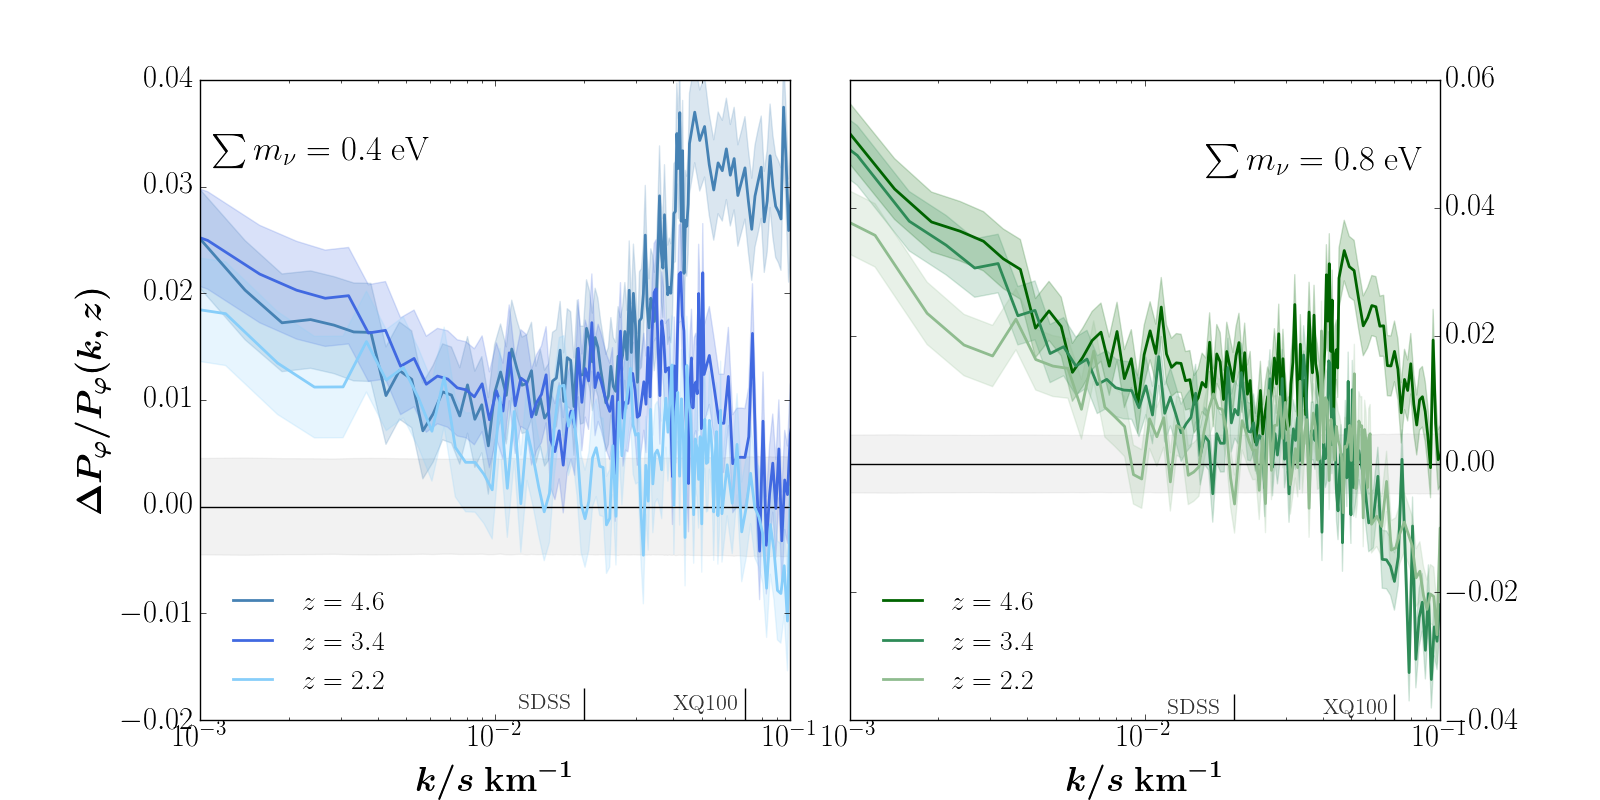
\includegraphics[width=\columnwidth]{Mnu/Mnu_Pf.png}
\caption{Relative difference in flux power spectrum with respect to the central \textit{best guess} model (black line) for $\sum m_\nu / \mathrm{eV} = 0.4$ (left) and $0.8$ (right). Uncertainty on $P_\varphi (k)$ is encoded in the shade thickness. Color encodes redshifts $z=2.2, 3.4$ and $4.6$. The `SDSS' and `XQ100' ticks refer to the highest data $k$ mode in each survey.}
\label{fig:flux_mnu_0408}
\end{center}
\end{figure}

In this final subsection, I recap the results on constraining active neutrino masses with Ly-$\alpha$ forests. Technically, neutrinos are hot dark matter, since we know from the cosmic microwave background and particle physics experiments that their effective mass lies below the $\lesssim \mathrm{eV}$ scale. Fig.~\ref{fig:visu_wdm} illustrates the effect of free-streaming of warm dark matter particles, as they delay the formation of large scale structures on increasingly large characteristic length as the mass of the particle decreases (equivalently, their thermal velocities increases). Particles lighter than $\lesssim \mathrm{keV}$ delay the formation of galaxies to too late cosmological times to be consistent with observational data. As such, sub-eV neutrinos cannot account for all of dark matter. Just as I investigated warm dark matter particles as a partial component of the dark matter population\footnote{assuming that dark matter is made of particles}, one can consider $\omega_\nu ~=~ F_{\mathrm{hdm}} ~\omega_{\mathrm{dm}}$ with $0 \leqslant F_{\mathrm{hdm}} \leqslant 1$ the relative abundance of neutrinos with respect to the total dark matter density, the complementary component once again being generically and undeterminedly cold. Unlike the C+WDM cosmologies, the actual background density of neutrinos is known. Because of their light masses, neutrinos spend a certain amount of time behaving like radiation still well within the Matter Dominated Era before becoming non-relativistic. As such, it is more relevant to quantify the relative abundance of neutrinos with respect to the matter component $0 < f_\nu \leqslant 1$ such that $\Omega_\nu = f_\nu \Omega_m = f_\nu ( \Omega_\nu + \Omega_b + \Omega_{\mathrm{dm}} )$, which was introduced in Eq.~\ref{eq:f_nu}. Although $f_\nu$ and $F_{\mathrm{hdm}}$ can be trivially linked, I choose to express the relative abundance of neutrinos with the former for the sake of consistency with the literature and its historical groundings. In fact, when neutrinos as dark matter was initially investigated in the 70's, there was no evidence for dark energy and the critical density of the Universe was defined such that $\Omega_m = 1$ for a Universe with no curvature. As such, $f_\nu = 1$ used to  correspond at that time to a Universe whose energy density is dominated by neutrinos. \\

In cosmology, the relevant observable on neutrino masses is the sum of their mass eigenstates $\Sigma m_\nu = m_1 + m_2 + m_3$. It is linked to the neutrino density by virtue of Eq.~\ref{eq:meff_link}, and as such, $\sum m_\nu \propto f_\nu$ controls the height of the small-scale plateau in the matter transfer function, at least in the linear regime (see Fig.~\ref{fig:pk_chdm} and Eq.~\ref{eq:tnu}). \\



\begin{table}
\begin{center}
\begin{tabular}{lccc}
\hline \\[-10pt]
\textbf{Data set} & \textbf{Ly-$\alpha$ + $H_0$} & \textbf{+ CMB} & \textbf{+BAO} \\[2pt]
\hline \\[-10pt]
BOSS DR9 & $1.1$ & $0.12$ & $0.12$ \\[2pt]
BOSS DR9 + XQ-100 & $0.8$ & $0.14$ & $0.14$ \\[2pt]
\hline \\[-10pt]
\end{tabular}
\end{center}
\caption{$95\%$ C.L. upper bounds on $\Sigma_\nu$ in units of eV. `Ly-$\alpha$ + $H_0$' refers to the 1D power spectrum from the Ly-$\alpha$ forest in addition to the Gaussian prior on $H_0 = 67.3 \pm 1.0~\mathrm{km}~s^{-1}\mathrm{Mpc}^{-1}$ from Planck. The `CMB' refers to the Planck 2015 TT power spectrum and low$~\ell$ polarization. Addining `Ly-$\alpha$+$H_0$+CMB+BAO' is all the previously stated data sets, + the TE and EE power spectra from Planck and measurements of the baryon acoustic oscillations listed in Sec.~\ref{sec:data}}
\label{tab:Mnu_limits}
\end{table}



Fig.~\ref{fig:flux_mnu_0408} displays the (non-linear, unidimensional) Ly-$\alpha$ flux power spectrum for C+HDM cosmologies with $\Sigma m_\nu = 0.4$ and $0.8$ eV. Since the scales probed by the Ly-$\alpha$ forest are in the flat plateau regime of the matter transfer function, the free-streaming effect of neutrinos is correlated to the effect of $\Omega_m$, $\sigma_8$ or $n_s$ ($52 \%,~-48\%$ and $48\%$ correlation respectively). To lift the degeneracy between these parameters, in addition to computing the flux power spectrum for our whole grid of parameters, we make use of the CMB data from Planck, which tightly constrains the cosmological parameters $\left( \Omega_m, \sigma_8, n_s, h \right)$. Fig.~\ref{fig:c2d_om_sig} displays the $68\%$ and $95\%$ contours in the $\left( \Sigma m_\nu, \Omega_m \right)$ and $\left( \Sigma m_\nu, \sigma_8 \right)$ parameter spaces, with Ly-$\alpha$ forests (SDSS/BOSS) alone (in addition to a prior on the current expansion rate $h = 0.673 \pm 0.010$), combined BOSS and XQ-100, CMB (Planck) alone, and all of those probes combined. As visible in Fig.~\ref{fig:1d_scan}, our best fit falls in the $\sum m_\nu < 0$ (unphysical) region when using Ly-$\alpha$+$H_0$+CMB. When adding BAO, the best fit falls within the $\sum m_\nu > 0$ (physical) region. 
%However, the $\sum m_\nu \sim 0.045~\mathrm{eV}$ best fitted value is implausible since it is known from neutrino oscillations that at least one of the eigenstates is massive with $\Sigma m_\nu = m_1 \geqslant 0.06~\mathrm{eV}$. 
Tab.~\ref{tab:Mnu_limits} recaps our upper bounds on $\Sigma m_\nu / \mathrm{eV}$ in terms of the $95\%$ confidence level, using our available cosmological probes.

\begin{figure}
\begin{center}
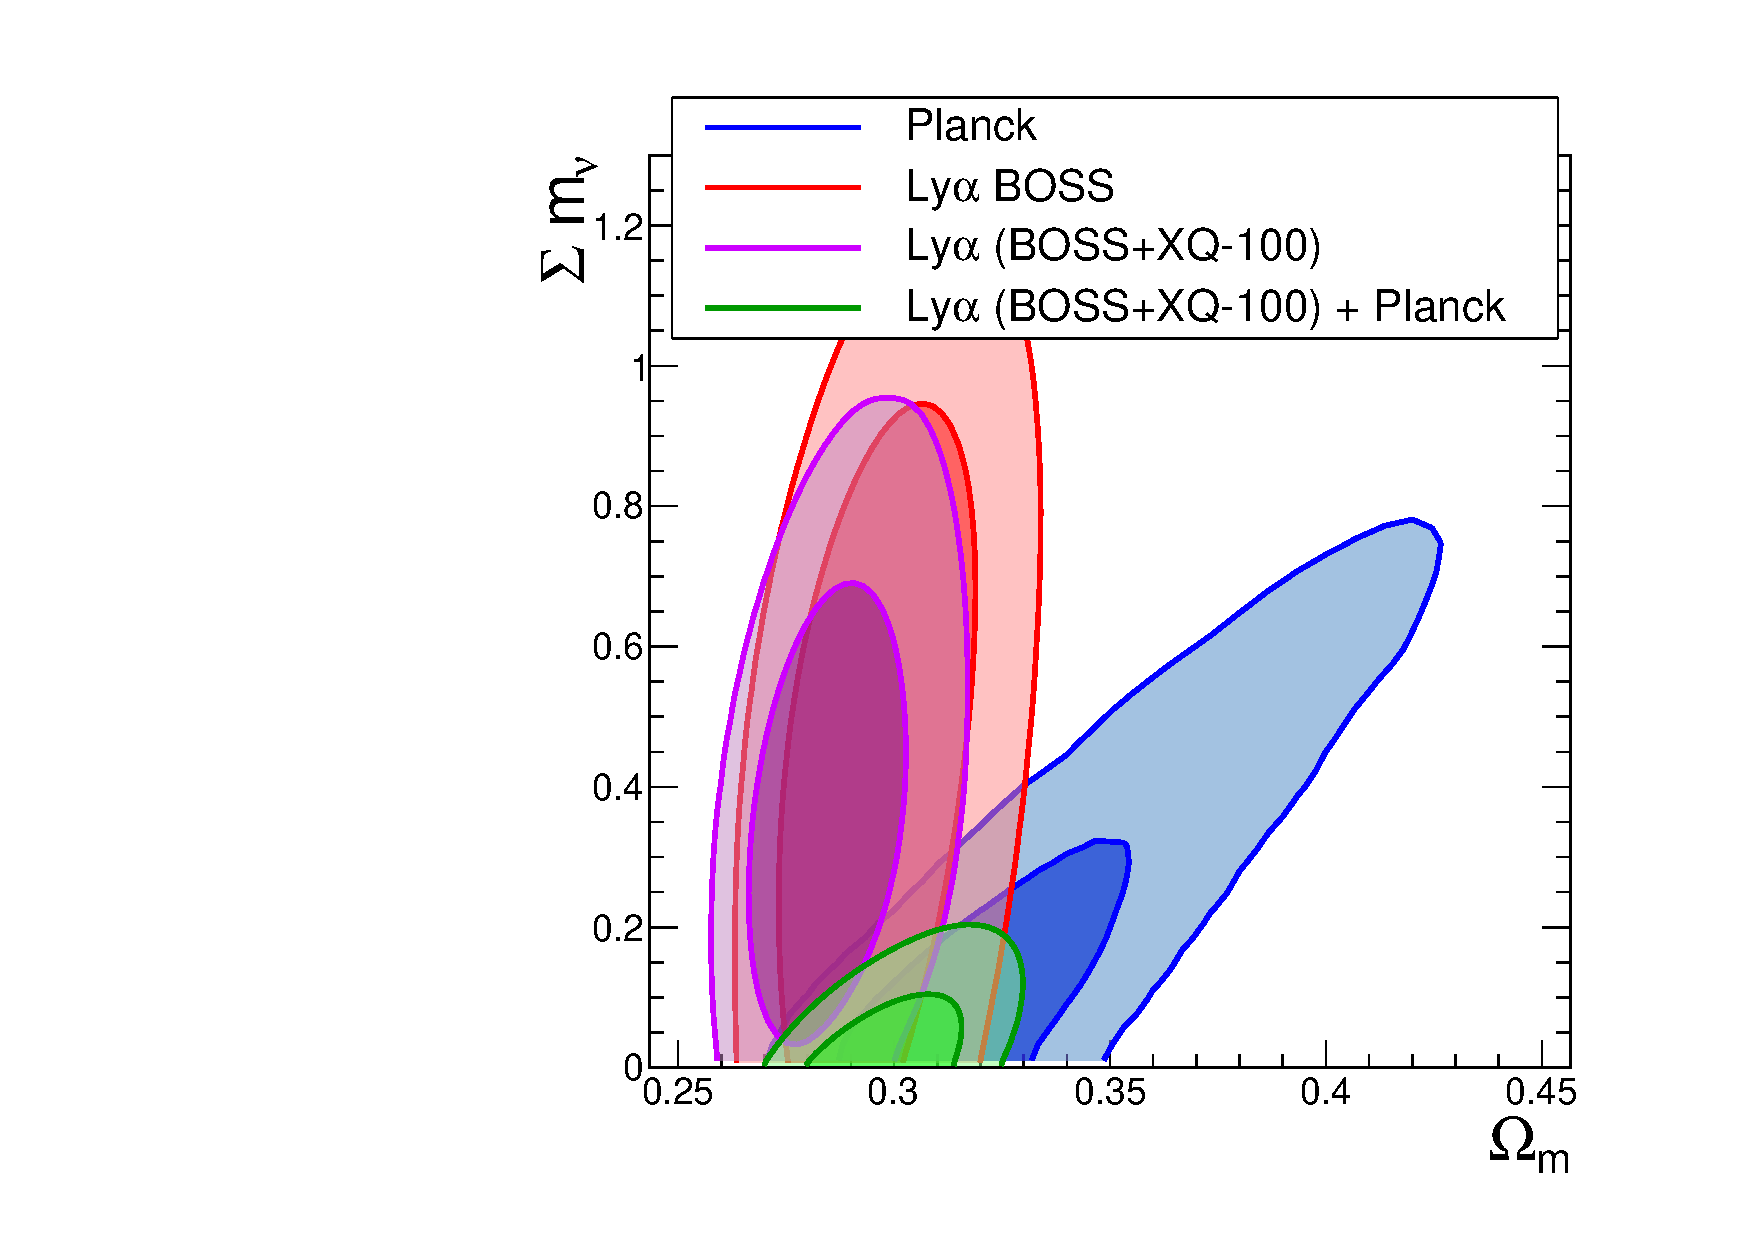
\includegraphics[width=0.55\columnwidth]{Mnu/OmegamMnu_Planck_Lya.pdf}~%
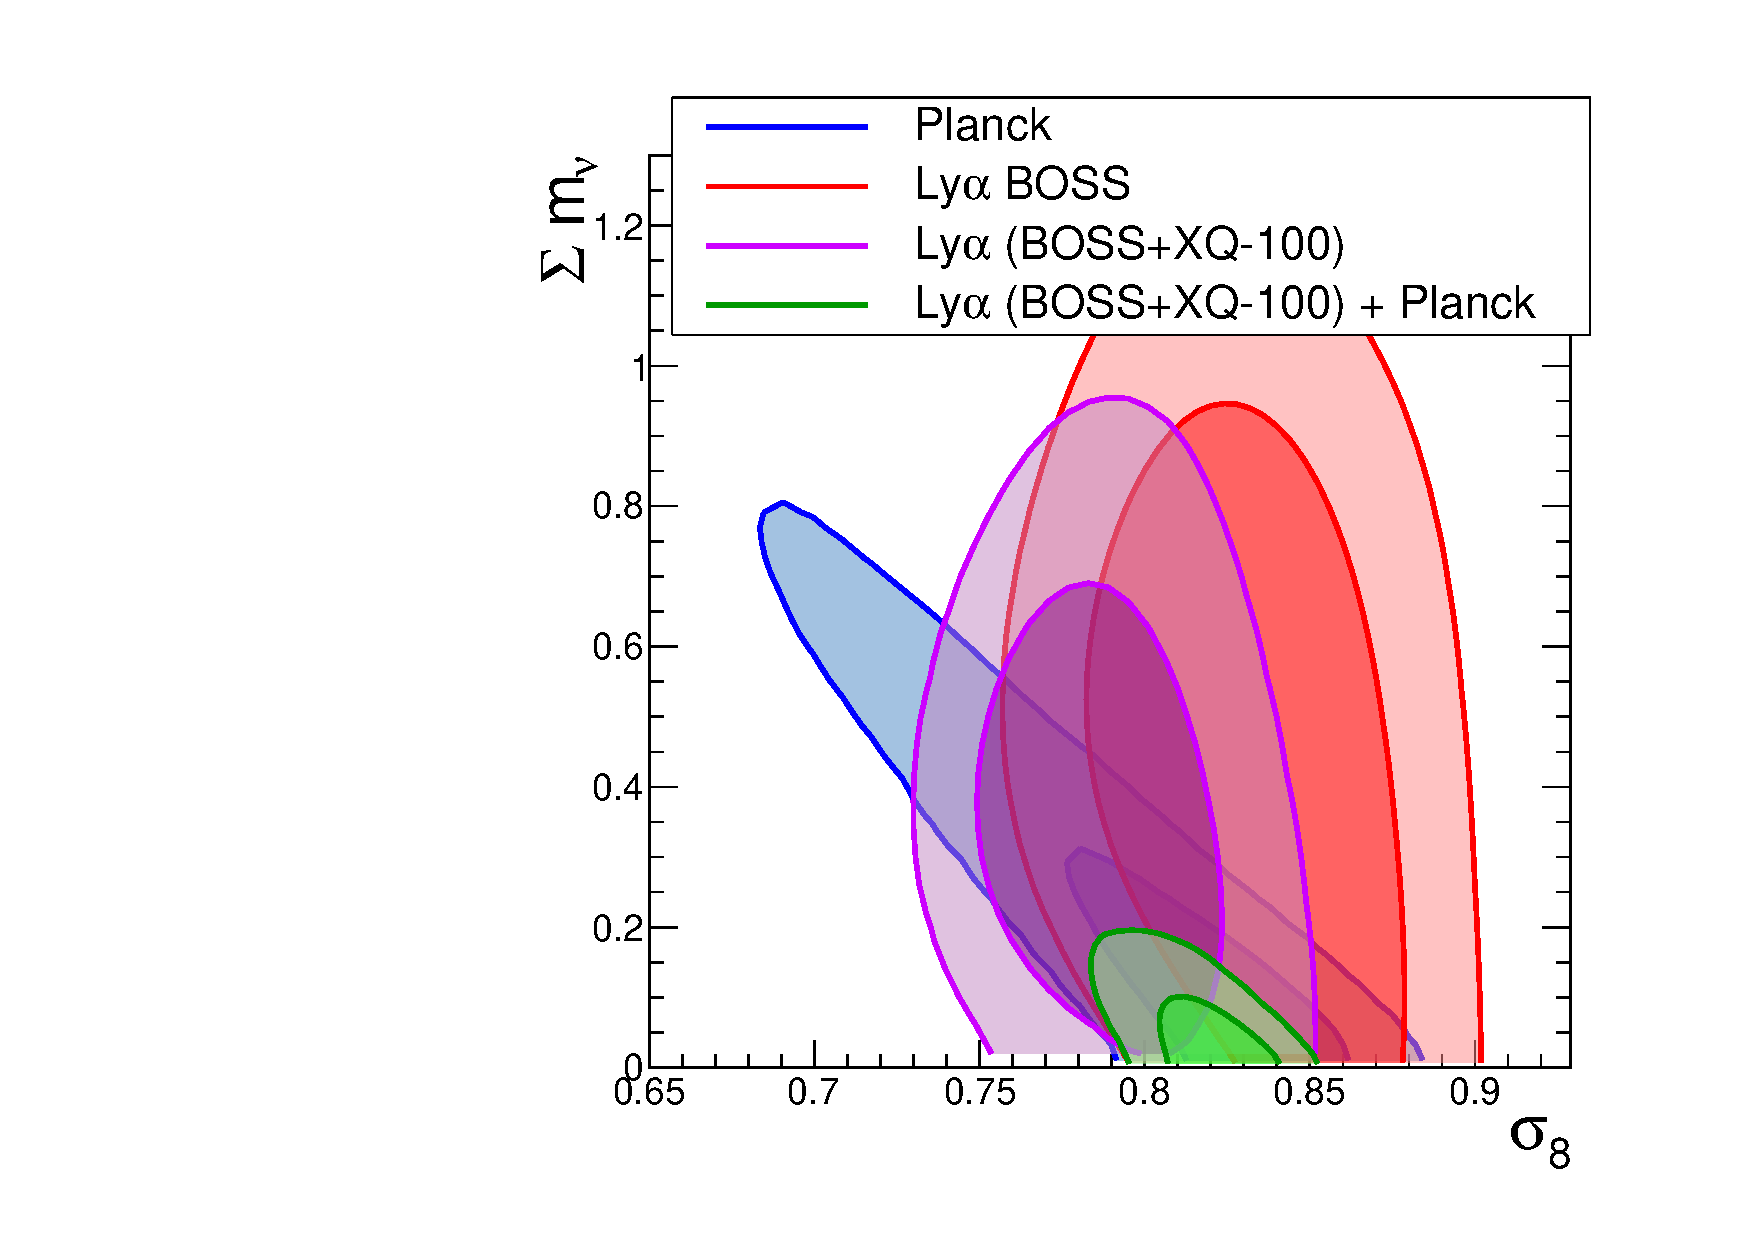
\includegraphics[width=0.55\columnwidth]{Mnu/sigma8_Mnu_Planck_Lya.pdf}
\caption{$68\%$ and $95\%$ C.L. in $\left( \sum m_\nu, \Omega_m \right)$ and $\left( \sum m_\nu, \sigma_8 \right)$ using BOSS only (red), BOSS+XQ100 (purple) for the Ly-$\alpha$+$H_0$ sets. Constraints from the Planck 2015 likelihood on CMB TT + low-$\ell$ data is featured in blue. Combining CMB and Ly-$\alpha$ forest data sets issues the constraints in green.}
\label{fig:c2d_om_sig}
\end{center}
\end{figure}


\begin{figure}
\begin{center}
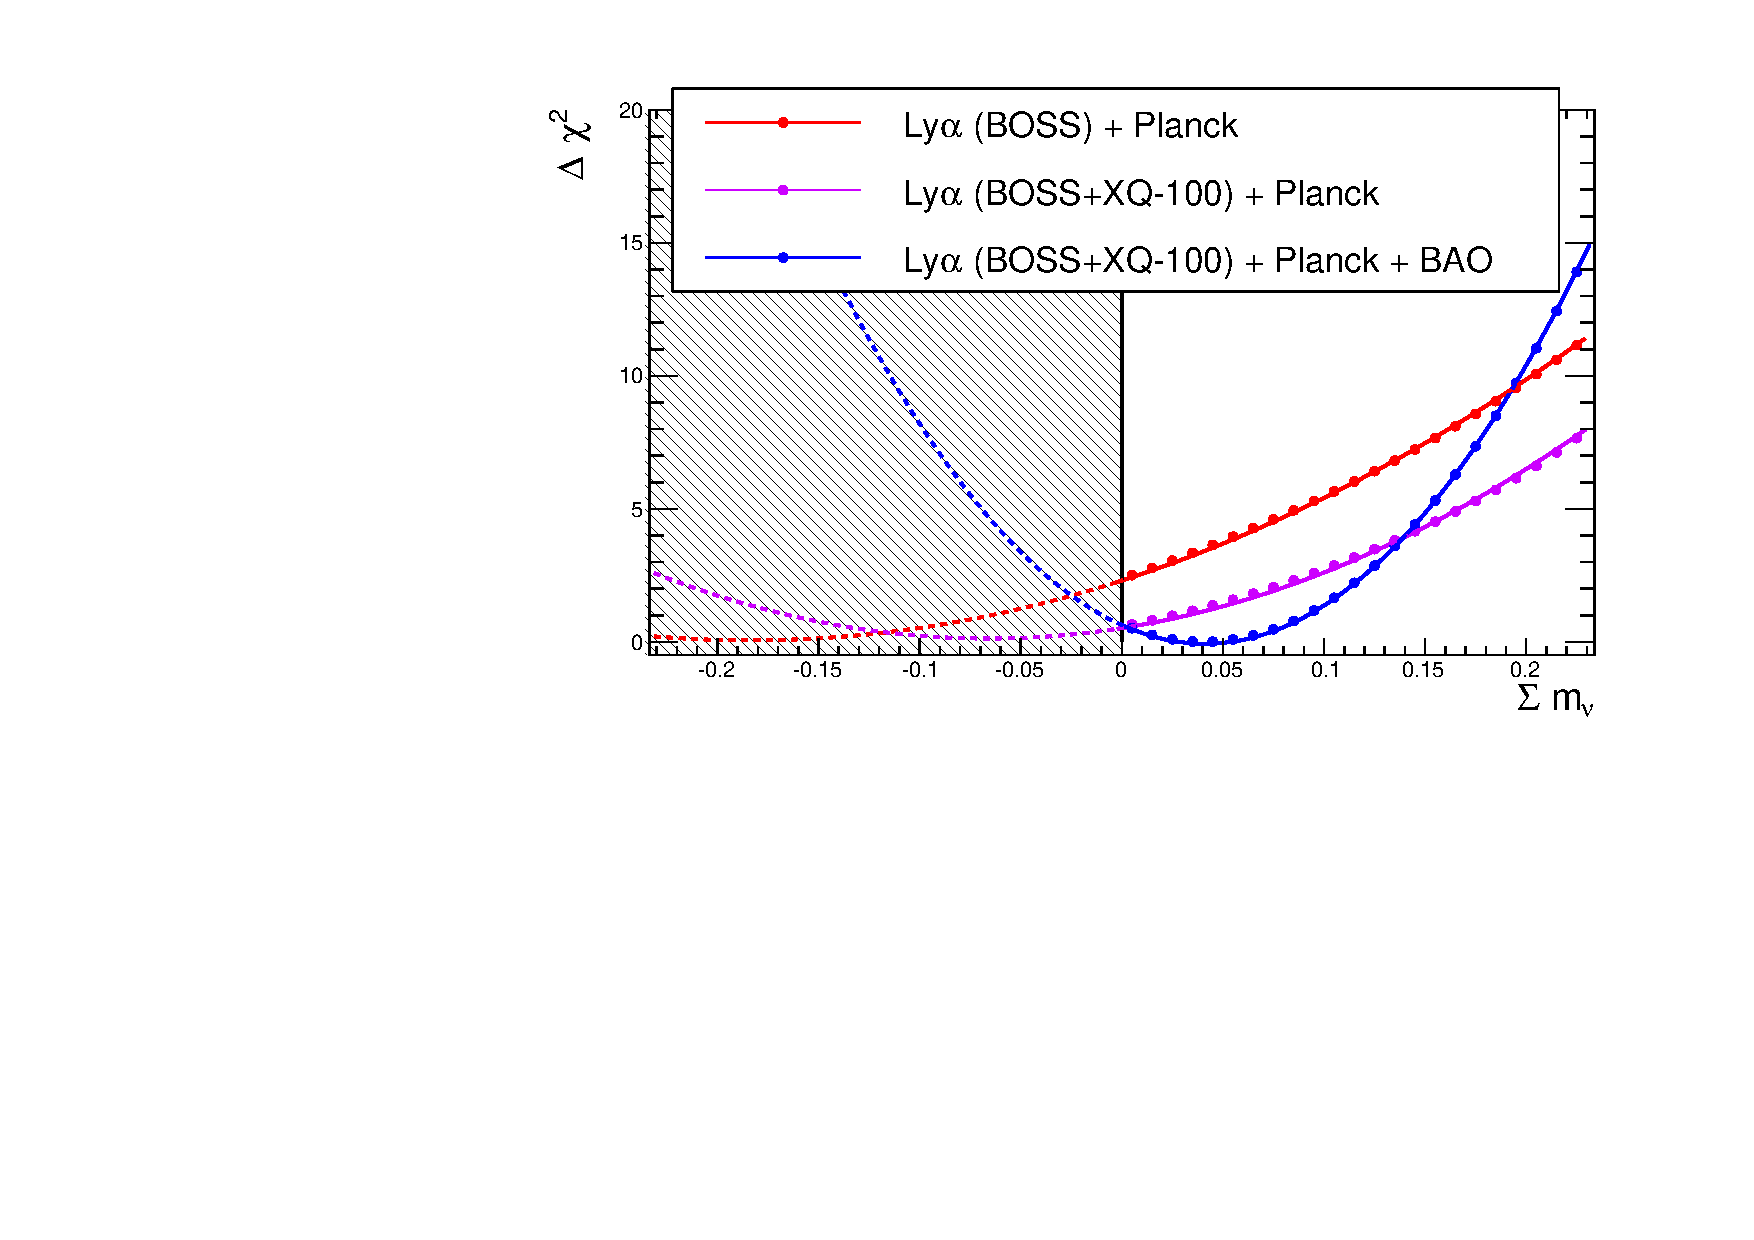
\includegraphics[width=0.85\columnwidth]{Mnu/Scan_1D_Chi2_Mnu.pdf}
\caption{$\chi^2$ profile with respect to $\sum m_\nu$}
\label{fig:1d_scan}
\end{center}
\end{figure}





\subsubsection{Discussion on $\sum m_\nu$ and $\mathrm{d} n_s / \mathrm{d} \ln k$}

The joint Ly$\alpha$ + CMB analysis presented in this work enables setting stringent constraints on cosmology, providing significant improvements upon CMB  alone from \cite{Planck2015} on two main fronts: the constraint on $\sum m_\nu$ is much tighter, and a running of $n_s$ is measured at more than $3~\sigma$. We here discuss these two results in terms of their robustness and correlations. \\

The constraint on $\sum m_\nu$, on the one hand, comes from the measurement of $\sigma_8$ in Ly$\alpha$ data, and from the correlation between $\sigma_8$ and $\sum m_\nu$ provided by the CMB. The value of $\sigma_8$ is derived from the normalization of the 1D flux power spectrum, and thus from its measurement at zeroth order. \\

The value of ${\mathrm d}n_s/{\mathrm d}\ln k$, on the other hand, is derived from the different values of $n_s$ determined by the CMB and the Ly$\alpha$ forest (\textit{e.g.} from the measurement of the 1D flux power spectrum at first order to access the slope information that determines $n_s$), and from variations of $n_s$ within the scales probed by either  probe (\textit{e.g.} from the measurement of the 1D flux power spectrum at second order). It is therefore more sensitive to systematic effects  in the measurement of the flux power spectrum. 
For instance, the slope of the 1D flux power spectrum is sensitive to  the modeling of  instrumental effects (such as spectrograph resolution) as well as of physical contributions (such as SN or AGN feedback, UV fluctuations, \textit{etc.}) affecting the IGM.  These effects have been included in this work through nuisance parameters that are fitted along with the relevant cosmological parameters. This is nevertheless a delicate task, not free of any possible yet-unaccounted-for additional systematic which could affect the determination of $n_s$. \\

In \cite{Palanque2015a} (Sec. 4.2.2), we showed that the impact of $\sum m_\nu$ on the $2.3\sigma$ tension on $n_s$ did not affect the result since the tension on $n_s$ is roughly the same for small (0.1 eV) or large (0.3 eV) neutrino masses. In \cite{Palanque2015b}, we infered a similar conclusion from the fact that $n_s$ and $\sum m_\nu$ have little correlation, both in Ly$\alpha$ and in CMB data. As a final test, we implemented a dedicated MCMC for CMB data, allowing both $\sum m_\nu$ and ${\mathrm d}n_s/{\mathrm d}\ln k$ to vary. The result indicates a null correlation between these two parameters. Errors or limits on both parameters are also in excellent agreement with the values obtained when only one of them at a time is included in the fit, confirming the absence of degeneracy between $\sum m_\nu$ and ${\mathrm d}n_s/{\mathrm d}\ln k$. 
In conclusion, if in future investigations a systematic effect that affects the determination of $n_s$ is found, it would directly alter the determination of ${\mathrm d}n_s/{\mathrm d}\ln k$ but would not modify significantly  the limit on $\sum m_\nu$.





\subsubsection{Impact of Mass Ordering}
\label{sec:ordering_impact}

\begin{figure}
\begin{center}
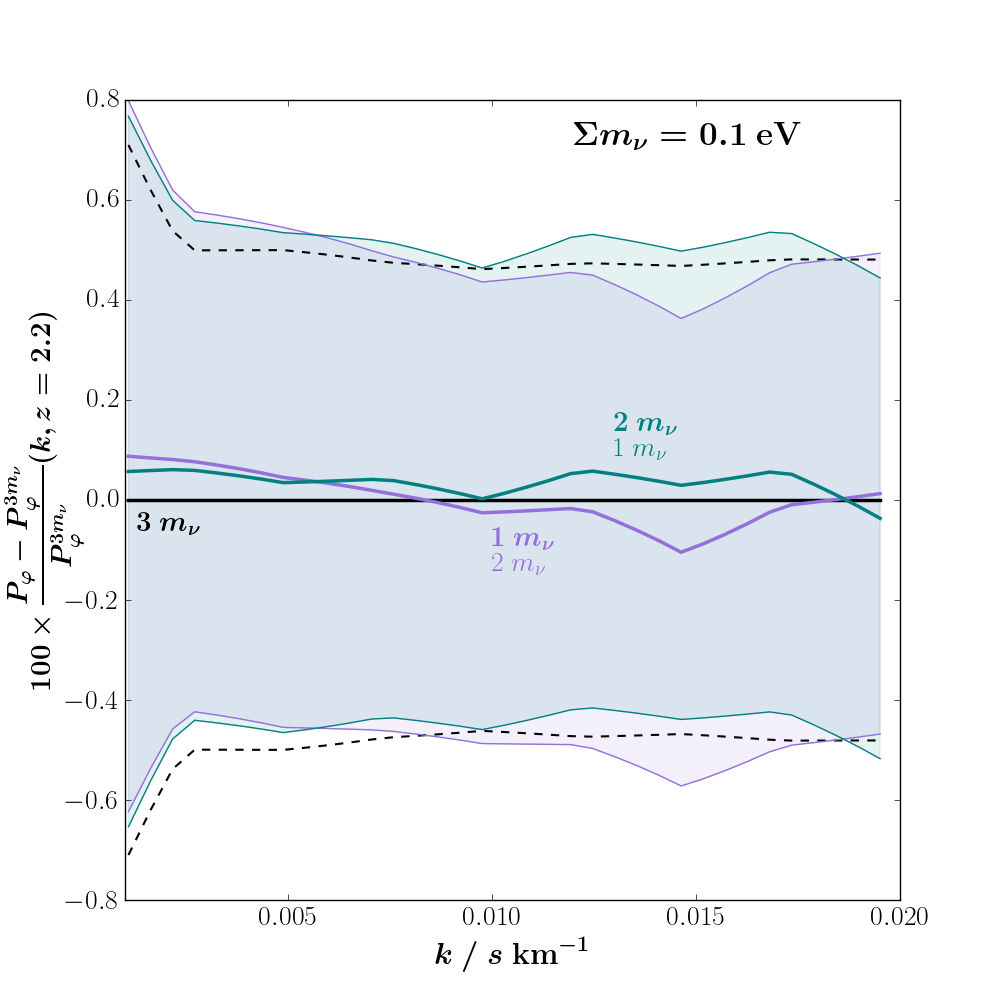
\includegraphics[width=0.85\columnwidth]{Ordering_Pflux_z22.png}
\caption{Relative difference in flux power spectrum at $z=2.2$ with $\sum m_\nu = 0.1~\mathrm{eV}$ of the normal (inverse) ordering in green (purple) with respect to three degenerate neutrinos (black line) in units of percent. Uncertainty on $P_\varphi (k)$ is encoded in the shade thickness.}
\label{fig:flux_ordering}
\end{center}
\end{figure}

In Sec.~\ref{sec:mass_ordering}, I layed out the difference in terms of the linear matter power spectrum of modeling a single neutrino of effective mass $\sum m_\nu$, three neutrinos degenerate in mass ($\sum m_\nu / 3$ each) and three neutrinos in a non-degenerate mass ordering: one heavy and two light states ``normal'' ordering) or one light and two heavy states ``inverted'' hierarchy). I pointed out in Fig.~\ref{fig:smnu_mnu} that for $\sim$eV neutrinos, the three eigenstates are for all intents and purposes degenerate. The atmospheric and solar squared mass differences only differentiate the three mass levels at the sub-eV scale, which is relevant for the values of $\sum m_\nu$ we investigate. The black vertical lines in Fig.~\ref{fig:smnu_mnu} indicate the values of $\sum m_\nu$ used in our suite of hydrodynamic simulations and for which we've construted the flux power spectrum: $0.2, 0.4$ and $0.8$ eV. One can see that the lighter the sum mass of neutrinos, the more disparate the ``solo'' from the ``degenerate'' configurations become, and one can even make out the difference between both ordering schemes, especially for $\sum m_\nu = 0.2~\mathrm{eV}$. I therefore investigated whether the mass ordering can be detected in our Ly-$\alpha$ power spectrum, and if not, how to model an additional systematic due to mass ordering. I do so by running three simulations and construct the flux power spectrum for the ``degenerate'', ``normal'' and ``inverted'' configurations for $\sum m_\nu = 0.1~\mathrm{eV}$. This corresponds to the limit case below which the inverted ordering is \textit{de facto} excluded (see Fig.~\ref{fig:smnu_mnu}). The two heaviest states in all three configurations are relatively equivalent. However, the two lightest states show significant differences of order unity, with the lightest state of the inverted ordering being essentially massless (see Tab.~\ref{tab:ordering}). Fig.~\ref{fig:pk_hierarchy} displays the linear matter transfer function for all three configurations for this specific (yet unrealistic) sum mass, in addition to the "solo" configuration (which is indistinguishable from three degenerate neutrinos). The relative difference between the three configurations is expected to be even lower than the fifth of a percent in the linear case since what is displayed in Fig.~\ref{fig:pk_hierarchy} is the three-dimensional transfer function. When integrating along parallel $k$ modes to get the 1D transfer function, the relative difference is significantly attenuated. \\


The differences between orderings are even more attenuated when comparing their 1D flux power spectra. As shown in Fig.~\ref{fig:flux_ordering}, the ratio of the 1D flux power spectrum measured for inverted or normal orderings to the power spectrum for degenerate masses is compatible with 1 at better than 0.05\%, more than 10 times below the level of the statistical uncertainty in the simulations. The plot is centered on scales probed by the Ly$\alpha$ forest flux power spectrum from the SDSS/BOSS DR9 data set (see Sec.~\ref{sec:p1d}). This test clearly justifies the simplifying hypothesis of degenerate masses used in this work. The effects of individual neutrino masses are too small to be measured with current experiments or even with the next generation experiments like DESI.\\

\subsubsection{Implications for Particle Physics}

Here, I briefly discuss the implications of this investigation for the individual masses $(m_1,m_2,m_3)$ of the three neutrino mass eigenstates $(\nu_1,\nu_2,\nu_3)$.  The atmospheric, solar, reactor and accelerator neutrino experiments constrain two squared mass differences, $\Delta m^2_\mathrm{sol}$ and  $\Delta m^2_\mathrm{atm}$ (with $\Delta m^2_\mathrm{sol} \ll \Delta m^2_\mathrm{atm}$, following the formalism in~\cite{Capozzi2013csa}). Assuming one of the two mass orderings, our constraints on $\sum m_\nu$ allows one to derive direct constraints on the individual masses $(m_1,m_2,m_3)$. \\

We can compare these constraints to  direct measurements of the mass  $m_\beta$ with single $\beta$-decays as planned by the KATRIN experiment~\cite{Osipowicz2001sq} with tritium $\beta$-decay.  In absence of neutrino oscillations, this experiment would probe the reaction
$$ ^{3}{\rm H} \rightarrow \, ^{3}{\rm He} + e^- + \nu_e$$
However, what tritium $\beta$-decay experiments really probe is an incoherent sum of the three reactions
$$ ^{3}{\rm H} \rightarrow \, ^{3}{\rm He} + e^- + \nu_i$$
where $i \in \lbrace 1,2,3 \rbrace$ and $\nu_i$ the $i$ mass eigenstates. At currently achievable resolution, the measurable amplitude is therefore related to the combination  shown in Eq.~\ref{eq:numassbeta} where $U_{ei}$ are the 3 coefficients of the first line of the  Pontercorvo-Maki-Nakagawa-Sakata (PMNS)  mixing matrix.    
Indeed, this neutrino mass,  $m_\beta$, can be directly derived from the masses $(m_1,m_2,m_3)$  through the PMNS mixing matrix $U(\theta_{12}, \theta_{13},\theta_{23})$ where $\theta_{ij}$ are the mixing angles:
\begin{equation}
m_\beta =  \left( \sum_i |U_{ei}|^2 m_i^2 \right)^\frac{1}{2}=\left( c_{13}^2  c_{12}^2 m_1^2  +  c_{13}^2  s_{12}^2 m_2^2 +  s_{13}^2  m_3^2 \right)^\frac{1}{2}
\label{eq:numassbeta}
\end{equation}
with  $c_{ij}=\cos\theta_{ij}$ and $s_{ij}=\sin\theta_{ij}$. \\

The current upper limit on the ``effective electron neutrino mass'' $m_\beta$ is of the order of 2 eV. The  KATRIN experiment  will improve this limit by one order of magnitude down to 0.2 eV.  Figure~\ref{fig:ContourNuMass}  shows the values of $m_\beta$ that are consistent with the bounds on   $\sum m_\nu$ given in this work and with the constraints on $\delta m^2$, $\Delta m^2$, $s_{12}^2$ and $s_{13}^2$ derived by~\cite{Capozzi2013csa} from  the combination of atmospheric, solar, reactor and accelerator neutrino experiments, for both individual mass orderings. Combined with the contours from~\cite{Capozzi2013csa}, our results
imply $m_\beta<0.06$~eV  (respectively $m_\beta<0.04$~eV) for the inverted (\textit{resp.} normal) ordering.
A detection by Katrin of $m_\beta>0.2$~eV would thus call into question
the three-neutrino model used to interpret neutrino oscillation experiments. 


\begin{figure}
\begin{center}
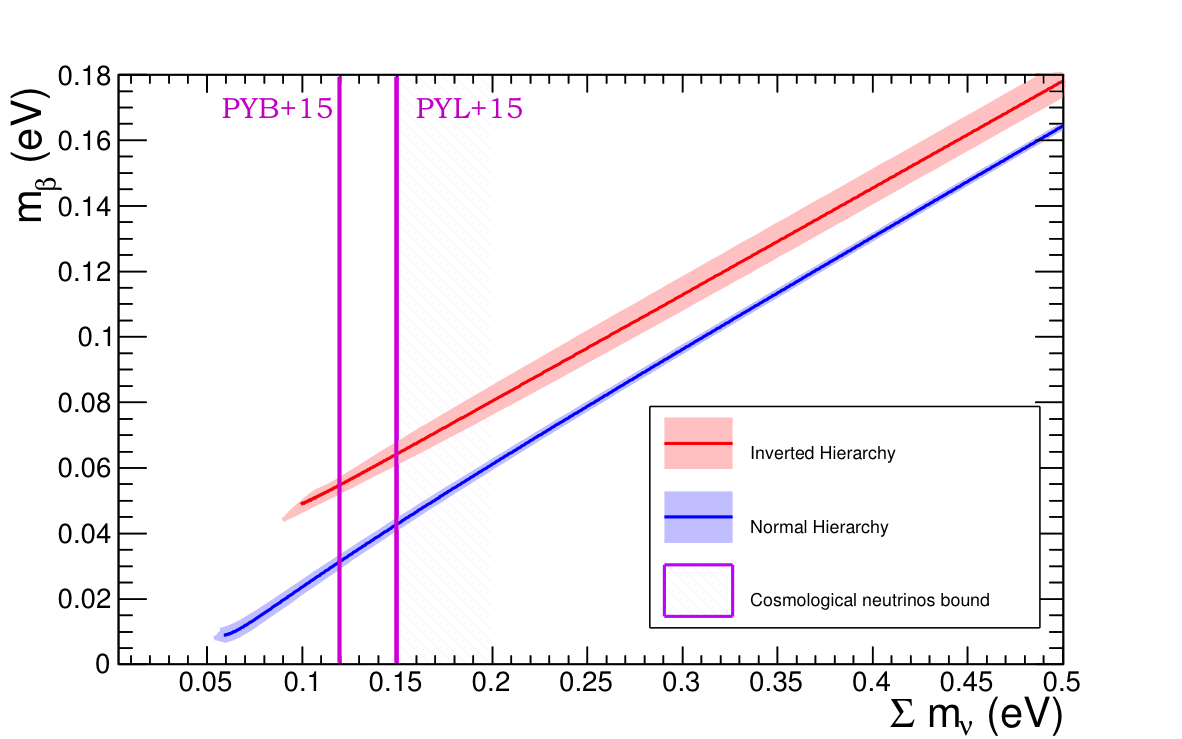
\includegraphics[width=0.85\columnwidth]{mnu_limits.png}
\caption{Constraints on the sum of the neutrino masses and the effective electron neutrino mass, $m_\beta$. The blue and red curves correspond, respectively, to the normal and inverted orderings obtained with the atmospheric, solar, reactor and accelerator neutrino experiments. The blue and red contours represent the $95\%$ C.L. derived from~\cite{Capozzi2013csa} around the central value of their fit. The purple hashed region represents the $95\%$ C.L. bound computed in \cite{Palanque2015a} (`PYL+15') and \cite{Palanque2015b} (`PYB+15', and this manuscript).}
\label{fig:ContourNuMass}
\end{center}
\end{figure}

